Tras establecer los parámetros necesarios correspondientes a la gestión del proyecto, este capítulo presenta el diseño del sistema implementado. Para ello se introducirá la estructura de directorios utilizada, el diagrama del software desarrollado y la gestión de las herramientas con el protocolo MCP. 

\section{Estructura del proyecto}
El proyecto se divide en cuatro contenedores separados, cada uno con su propio entorno virtual de python venv. La figura \ref{fig:dir_principales} muestra un resumen de los directorios: 

\begin{figure}[h]
\centering
\definecolor{folderbg}{RGB}{124,166,198}
\definecolor{folderborder}{RGB}{110,144,169}
\newlength\Size
\setlength\Size{4pt}
\tikzset{%
  folder/.pic={%
    \filldraw [draw=folderborder, top color=folderbg!50, bottom color=folderbg] (-1.05*\Size,0.2\Size+5pt) rectangle ++(.75*\Size,-0.2\Size-5pt);
    \filldraw [draw=folderborder, top color=folderbg!50, bottom color=folderbg] (-1.15*\Size,-\Size) rectangle (1.15*\Size,\Size);
  },
  file/.pic={%
    \filldraw [draw=folderborder, top color=folderbg!5, bottom color=folderbg!10] (-\Size,.4*\Size+5pt) coordinate (a) |- (\Size,-1.2*\Size) coordinate (b) -- ++(0,1.6*\Size) coordinate (c) -- ++(-5pt,5pt) coordinate (d) -- cycle (d) |- (c) ;
  },
}
\forestset{%
  declare autowrapped toks={pic me}{},
  declare boolean register={pic root},
  pic root=0,
  pic dir tree/.style={%
    for tree={%
      folder,
      font=\ttfamily,
      grow'=0,
    },
    before typesetting nodes={%
      for tree={%
        edge label+/.option={pic me},
      },
      if pic root={
        tikz+={
          \pic at ([xshift=\Size].west) {folder};
        },
        align={l}
      }{},
    },
  },
  pic me set/.code n args=2{%
    \forestset{%
      #1/.style={%
        inner xsep=2\Size,
        pic me={pic {#2}},
      }
    }
  },
  pic me set={directory}{folder},
  pic me set={file}{file},
}
\begin{forest}
  pic dir tree,
  pic root,
  for tree={% folder icons by default; override using file for file icons
    directory,
  },
  [tfg\_agentes\_software
    [sistema\_agentes
    ]
    [servidor\_mcp\_bd\_codigo
    ]
    [servidor\_mcp\_confluence
    ]
    [servidor\_mcp\_google\_drive
    ]
  ]
\end{forest}
\caption{Estructura de directorios principales del proyecto}
\label{fig:dir_principales}
\end{figure}


El directorio \textit{sistema\_agentes} contiene todos los agentes desarrollados y los clientes MCP. Los directorios \textit{servidor\_mcp\_bd\_codigo}, \textit{servidor\_mcp\_confluence} y \textit{servidor\_mcp\_google\_drive} contienen cada uno un servidor MCP de ejecución independiente. Para el desarrollo se han implementado 5 servidores MCP:

\begin{itemize}
\item \textbf{Servidores con protocolo SSE}: código del proyecto software y Confluence. Estos se alojan en contenedores separados ya que el protocolo SSE permite desacoplar el cliente MCP del servidor.

\item \textbf{Servidores con protocolo STDIO}: GitLab, Google Drive y sistema de ficheros local. La lógica de estos se he implementado junto a los agentes en \textit{sistema\_agentes} como se explica en la sección \ref{}. El servidor de Google Drive se mantiene en un contenedor independiente por ser una modificación de un repositorio no oficial: \url{https://github.com/felores/gdrive-mcp-server/blob/main/index.ts}.
\end{itemize}

\section{Diseño de agentes}

LangGraph proporciona un marco de trabajo estructurado para la creación de flujos de ejecución en forma de grafo. Se construye inicialmente un grafo mediante el objeto StateGraph, el cual establece la lógica de enrutamiento entre diversos nodos definidos como funciones de Python. Estos grafos utilizan un denominado estado, representado por un diccionario tipado, para almacenar el estado de ejecución durante el proceso.

Bajo este paradigma, un agente puede representarse como un grafo compilado, donde uno o varios nodos definen la lógica de invocación a los modelos LLM, mientras que otros nodos se encargan de interpretar el resultado. En una implementación tradicional, el estado conservaría los mensajes generados entre llamadas, lo que posibilita un proceso iterativo en el cual el nodo de invocación al LLM se ejecuta repetidamente, añadiendo un nuevo mensaje al estado en cada ciclo de ejecución.

Este enfoque proporciona un marco de trabajo orientado a la composición, puesto que un nodo puede constituir a su vez otro grafo compilado que represente a otro agente. Sin embargo, presenta una problemática de redundancia: cuando dos agentes comparten gran parte del grafo que los compone, para evitar la duplicación de código sería necesario desarrollar un grafo que contemple la ejecución de ambos tipos de agentes, determinando en cada instancia cuál ejecutar en función de un parámetro presente en el estado. Aunque esta solución es viable, la programación orientada a objetos ofrece una alternativa más elegante: la herencia.

Es por este motivo que se ha optado por un enfoque híbrido que combina composición y herencia. Cada agente está implementado mediante una clase de Python, la cual contiene una función que compone el grafo representativo de la ejecución del agente. De esta manera, la clase del agente define las funciones que representan cada nodo del grafo, pudiendo heredar aquellas definidas en clases más abstractas.

Adicionalmente, esta metodología facilita el almacenamiento de datos no vinculados a la ejecución individual. Los datos encapsulados en los atributos de las clases representan información invariable en cada ejemplo de ejecución, como el nombre del agente o las herramientas disponibles; mientras que los atributos almacenados en el estado del grafo son específicos de la ejecución, como los mensajes generados durante la instancia de ejecución concreta.

\subsection{Diagrama de agentes}

\begin{figure}[h]
  \centering
  \adjustbox{center=\textwidth}{\hspace{1cm}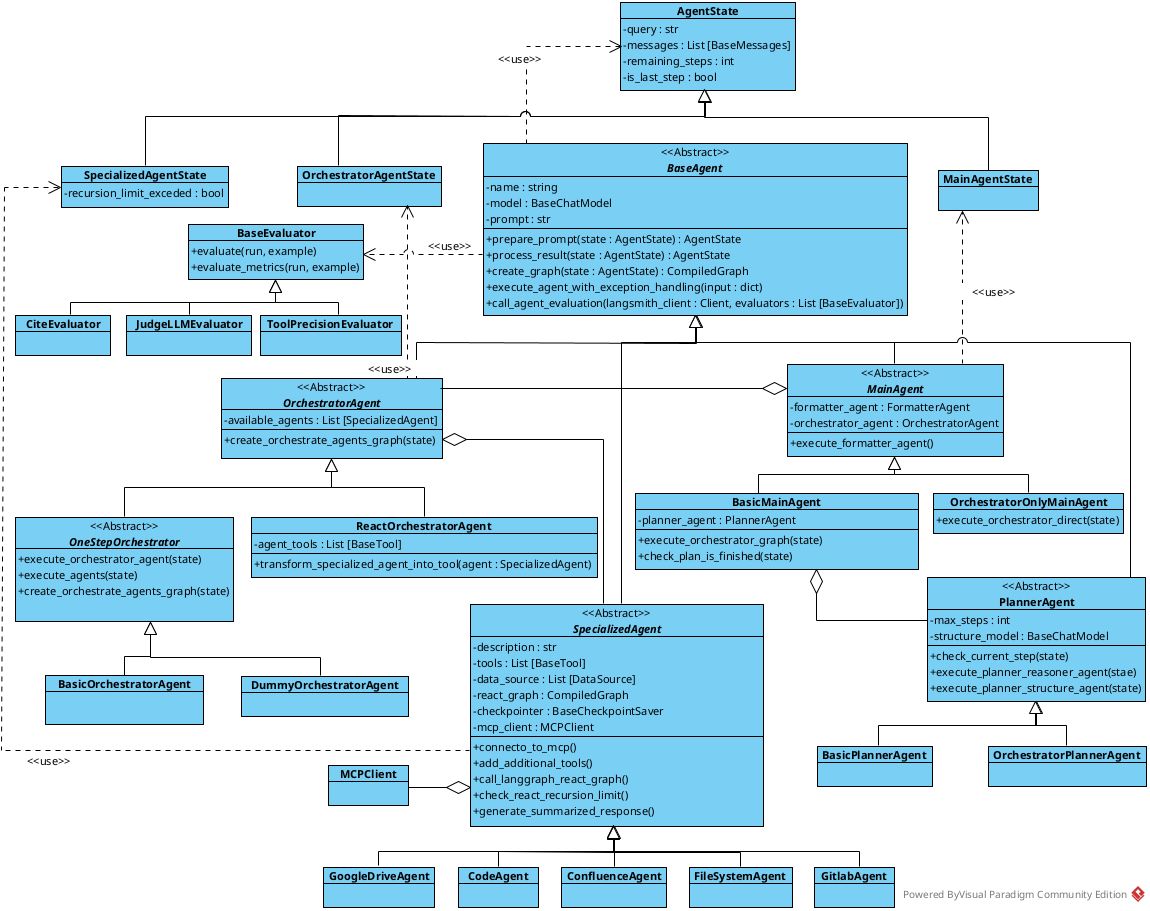
\includegraphics[width=1.35\linewidth]{figures/agentes.png}}
  \caption{Diagrama de clases UML de del sistema de agentes.}
  \label{fig:uml}
\end{figure}

La figura \ref{fig:uml} muestra el diagrama de clases general del sistema. La clase abstracta \textit{BaseAgent} define las funcionalidades básicas de todos los agentes: 
\begin{itemize}
  \item\textbf{Lógica de ejecución: }La función \textit{execute\_agent\_with\_exception\_handling} se encarga de invocar el grafo definido en \textit{create\_graph}, gestionando las excepciones e indicando los parámetros de entrada. Todos los agentes deben implementar la función \textit{prepare\_prompt}, e incluirla en su grafo de ejecución.
  \item\textbf{Gestión del resultado: }La función \textit{process\_result} se encarga de estáticamente devolver el resultado de ejeución del agente para dado un estado de ejecución. 
  \item\textbf{Evaluación del agente }La función \textit{call\_agent\_evaluation} se encarga en cada caso de definir la lógica de evaluación utilizando las métricas indicadas para cada agentes, representadas por la clase \textit{BaseEvaluator}. El capítulo \textbf{ref} explica este proceso en detalle.
\end{itemize}


Los agentes que heredan del agente base son los siguientes:
\begin{itemize}
  \item\textbf{SpecializedAgent: }Representa a los agentes que buscan en las fuentes de información especializadas, se explica en detalle en la sección \textbf{ref}. Define la lógica de gestión de las herramientas utilizadas mediante el cliente mcp, utilizando la clase Singleton \textit{MCPClient}, la cual encapsula la lógica de conexión con todos los servidores MCP disponibles, explicado en la sección \textbf{ref}. También contiene una secuencia de instancias de \textit{DataSource}, las cuales definen todos los documentos citables en las fuentes de datos disponibles, véase la sección \textbf{ref}.
  \item\textbf{OrchestratorAgent: }Implementa la lógica de enrutamiento de los agentes especialistas, decidiendo en cada caso cuáles agentes utilizar para una questión dada. Véase la sección \textbf{ref}. 
  \item\textbf{PlannerAgent: }Define la lógica de planificación a seguir para una consulta dada, creando planes secuenciales dinámicamente ajustables. Véase la sección \textbf{ref}.
  \item\textbf{FormatterAgent: }Convierte una secuencia de ejecución de agentes en un resultado legible, compuesta por una respuesta en formato textual y un conjunto de citas referenciando a documentos del proyecto software. Véase sección \textbf{ref}.
  \item\textbf{MainAgent: }Define el flujo general de la ejecución, especificando si se usarán agentes planfiicadores, orquestadores y concatenando su respueta al agente formateador. Véase la sección \textbf{ref}. 
\end{itemize}

Cada agente define su clase de estado, añadiendo en cada caso los atributos propios a la clase común \textit{AgentState}.

\section{Conexión Model Context Protocol (MCP)}

